\documentclass{siproblemset}

% SI Session Information
\course{MTH 1321}       % the course of your SI
\sessionnum{23}         % (optional) specify the session number
\sessiondate{4/16/20}   % the date of the session

\warmup{Concept Review}
\topic{Fundamental Theorem of Calculus, Part II}
\topic{FTOCII and Graphs}
\cooldown{Helpful Derivations}
%\topic{Net Change as Integrals of Rates of Change}
%\topic{$u$-substitution}

% Worksheet Information
\title{FTOCII}
\sections{Section 5.5}
\withnamespace

\newcommand{\dx}{\text{d}x}

\begin{document}
    \maketitle
    
    \activity{Warmup}{Concept Review}{Work \textbf{alone} to answer these questions. Try not to use your notes.}{15 minutes}
    
    \frq{What is the Fundamental Theorem of Calculus, Part II?}
    \smallsp
    
    \frq{What is the area/accumulation function?}
    \smallsp
   
    \activity{Activity 1}{Fundamental Theorem of Calculus, Part II}{Make a \textbf{group of two or three, all with the same colored worksheets}, to work together to answer these questions. Try not to use your notes. \textbf{DO NOT use a calculator}.}{30 minutes}
    \mcq{Use FTOCI to find the explicit formula for the area function represented by the following integrals.}{
        \task $\int_{4}^{x}e^{3u}\dd u$
        \smallsp
        \task $\int_{x}^{0}2^{-t}\dd t$
        \normalsp
    }
    \mcq{Compute the following derivatives.}{
        \task $\dddf t\int_{0}^{t}x^4-7x^2\dx$
        \Normalsp
        \task $\dddf s\int_{100}^{s}\ln(6u-5)\dd u$
        \Normalsp
        \task $\dddf s\int_{2}^{s}\sin(5t)\dd t$
        \Normalsp
    }
\newpage
    \mcq{Compute the following derivatives.}{
        \task $\dddf x\int_{0}^{x^2}\frac{t\dd t}{t+1}$
        \Normalsp
        \task $\dddf t\int_{-4}^{\sec(t)}u^3\dd u$
        \Normalsp
        \task $\dddf t\int_{-4}^{\sec(t)}u^3\dd u$
        \Normalsp
    }

    \newpage
    \activity{Activity 2}{FTOCII and Graphs}{Make a \textbf{group of two or three, all with the differently-colored worksheets}, to work together to answer these questions. Try not to use your notes. \textbf{DO NOT use a calculator}.}{30 minutes}
    
    \begin{multipartquestion}
        Let $A(x)=\int_0^xf(t)\text{d}t$. Use the graph of $f(x)$ below to answer the following questions. 
        \makebox[\width][c]{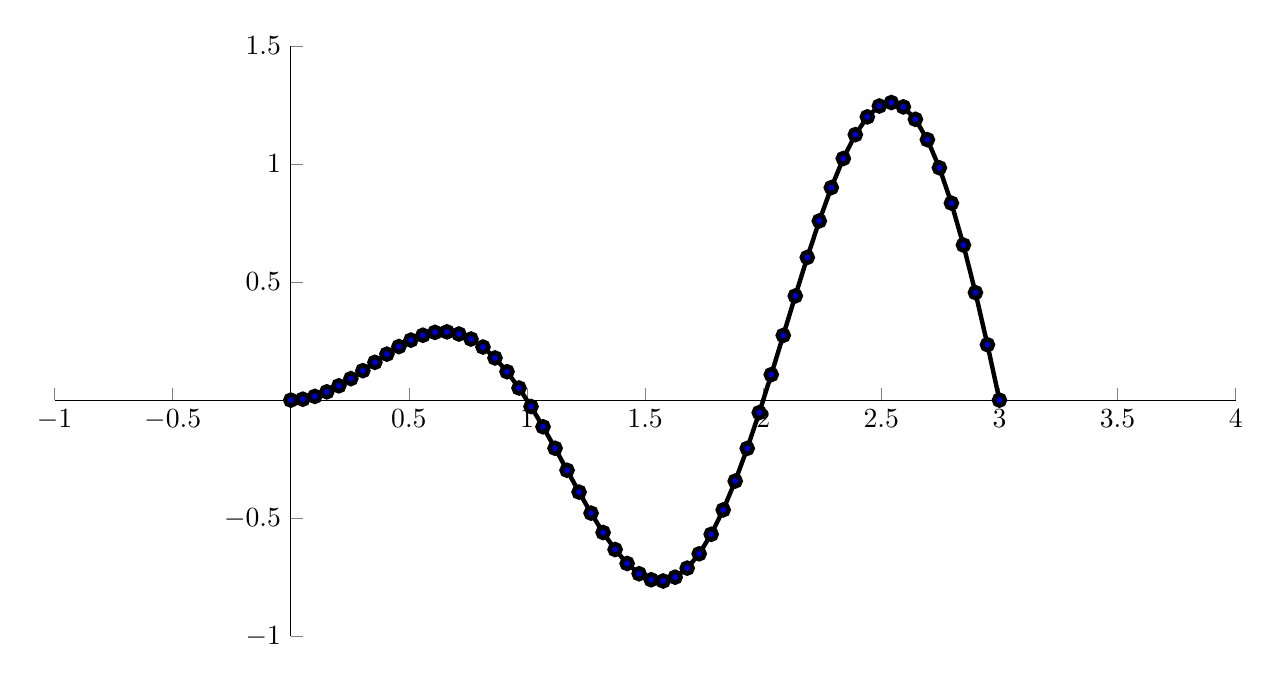
\begin{tikzpicture}[baseline=(current bounding box.north)]
            \begin{axis}[
            x=3cm,
            y=3cm,
            xmin=-1,
            xmax=4,
            ymin=-1,
            ymax=1.5,
            axis x line*=middle,
            axis y line*=middle,
            every axis plot/.append style={ultra thick},
            samples=60
            ]
            \addplot+[black, domain=0:3] {sin(180*x)*x/2};
            \end{axis}
            \end{tikzpicture}} 
        
        \frq{What are the intervals of increase and decrease for $A$?}
        \smallsp
        \frq{What are the $x$-values where $A$ has a local extremum?}
        \smallsp
        \frq{Where is $A$ concave up and down?}
        \smallsp
    \end{multipartquestion}

\newpage
    \begin{multipartquestion}
        Let $B(x)=\int_2^xg(t)\text{d}t$. Use the graph of $g(x)$ below to compute the following quantities.
        \makebox[\width][c]{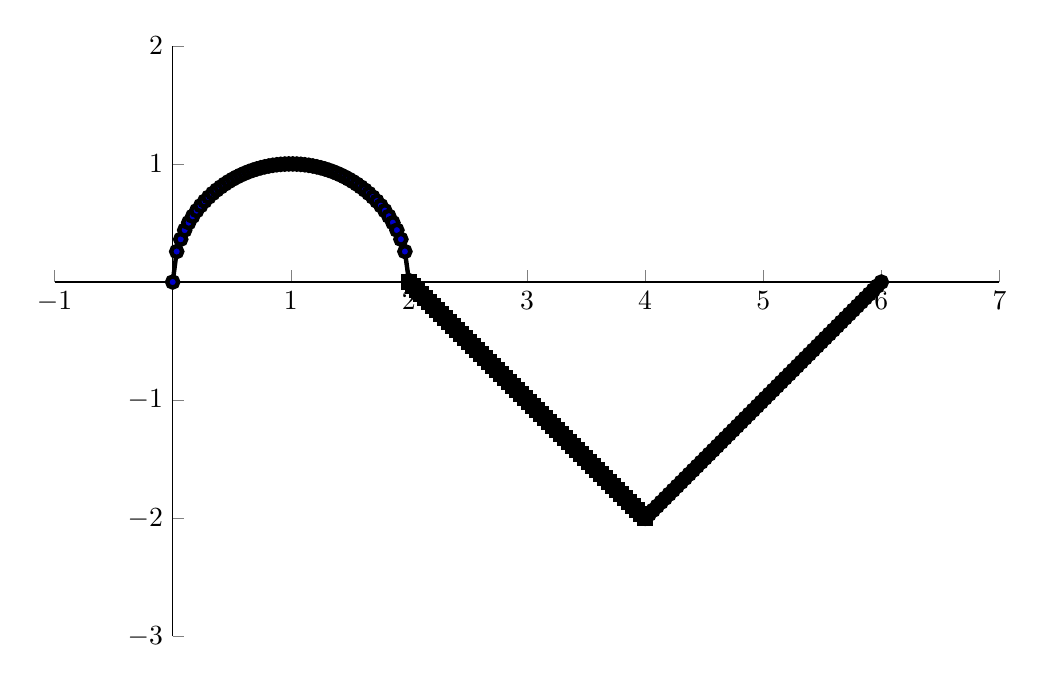
\begin{tikzpicture}[baseline=(current bounding box.north)]
            \begin{axis}[
            x=1.5cm,
            y=1.5cm,
            xmin=-1,
            xmax=7,
            ymin=-3,
            ymax=2,
            axis x line*=middle,
            axis y line*=middle,
            every axis plot/.append style={ultra thick},
            samples=60
            ]
            \addplot+[black, domain=0:2] {sqrt(1-(x-1)^2)};
            \addplot+[black, domain=2:4] {-x+2};
            \addplot+[black, domain=4:6] {x-6};
            \end{axis}
            \end{tikzpicture}}
        \frq{$B(0)$}
        \tinysp
        \frq{$B(2)$}
        \tinysp
        \frq{$B(6)$}
        \tinysp
        \frq{$B'(5)$}
        \smallsp
        \frq{$[B(5)]'$}
        \smallsp
    \end{multipartquestion}

\newpage
    \activity{Cooldown}{Helpful Derivations}{Make a \textbf{group of two or three, all with the differently-colored worksheets}, to work together to answer these questions. Try not to use your notes. \textbf{DO NOT use a calculator}.}{30 minutes}
    
    \frq{Derive an explicit expression for $\int_{a(x)}^{b(x)}f(t)\dd t$.}
    
\end{document}